\lstset{language=C}
\section{Session 4}


\subsection{Using Salome Meca}
\paragraph{}The first hour consisted on building the geometry of an \textsf{Y-pipe} with a software called \emph{Salome Meca}. A complete guide on video (with an older version of the program) can be found in:\\
\begin{center}
\url{http://caelinux.org/wiki/downloads/docs/Pipe2007/PipeGeom.htm}
\end{center}

\paragraph{}We open Salome by going to the folder that contains it, then we right-click on the \texttt{runAppli} file, select copy, and then select 'paste filename' in a terminal window. It should append the next command to the window\\
\lstinline!'/opt/salome_meca/appli_V2016/runAppli'!
\paragraph{}When we have our geometry constructed we have to export the files produced as \texttt{.stl} files. This files are based in a bunch of coordinates refering to the points of the piece. 
\subsection{Constructing the mesh}
\paragraph{}We want to make the mesh using \textbf{ParaView}. We can also use directly \emph{Salome-Meca} to mesh the pipe but its mesher is not as good as the one we're going to use. First we have to create a case. A good option is to look for a similar tutorial case as a basis for our mesh (and of course similar to the case we want to run). For the Y-pipe problem we can start with the motorbike case. To do so, create a folder and name it as Ypipe, then copy inside it the folders contained in the motorbike case. It can be done in a terminal by typing:
\begin{lstlisting}
	mkdir -p Ypipe
	cp -r /opt/openfoam4/tutorials/
	incompressible/simpleFoam/motorBike/* ./Ypipe
\end{lstlisting}

\paragraph{}Once we have the folder created the first we are going to do is to copy our geometry inside the case. (Copy the .stl an paste it in /constant/triSurface). The next step is  go to the  \texttt{system} folder, inside there is a file named \texttt{BlockMeshDict}. We must modify the block geometry to put the pipe inside it and mesh only the domain taht really interest us. The new values for the vertices of the block are:
\begin{center}
\begin{lstlisting}
vertices
(
    (-1 -2.5 -0.5)
    (3 -2.5 -0.5)
    (3  3 -0.5)
    (-1  3 -0.5)
    (-1 -2.5 0.5)
    (3 -2.5 0.5)
    (3  3 0.5)
    (-1  3 0.5)
);
\end{lstlisting}
\end{center}
\begin{figure}[h!]
\centering
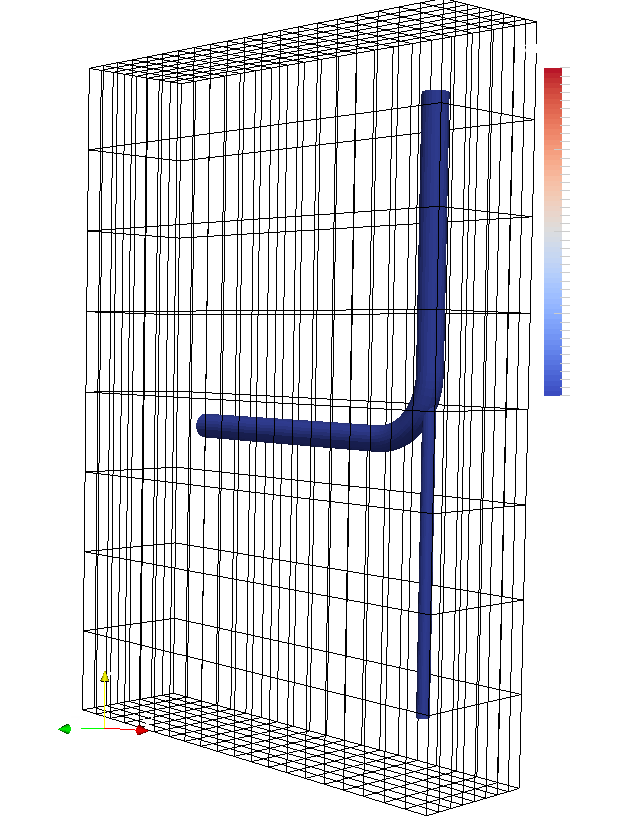
\includegraphics[scale=0.2]{mesh1.png}
\caption{First mesh. Toooooo coarse}
\end{figure}

\subsection{Refining the mesh}
\paragraph{}The next steps involve refining the mesh. To do so we are going to use \textbf{snappyHexMesh}(See reference). We must define the level 0 of the mesh. In this level we must have a mesh as regular as possible (squares in all 3 directions). Open \texttt{BlockMeshDict} an edit the following line:
\begin{center}
\begin{lstlisting}
blocks
(
    hex (0 1 2 3 4 5 6 7) (44 64 10) simpleGrading (1 1 1)
);
\end{lstlisting}
\end{center}
\begin{figure}[h!]
\centering
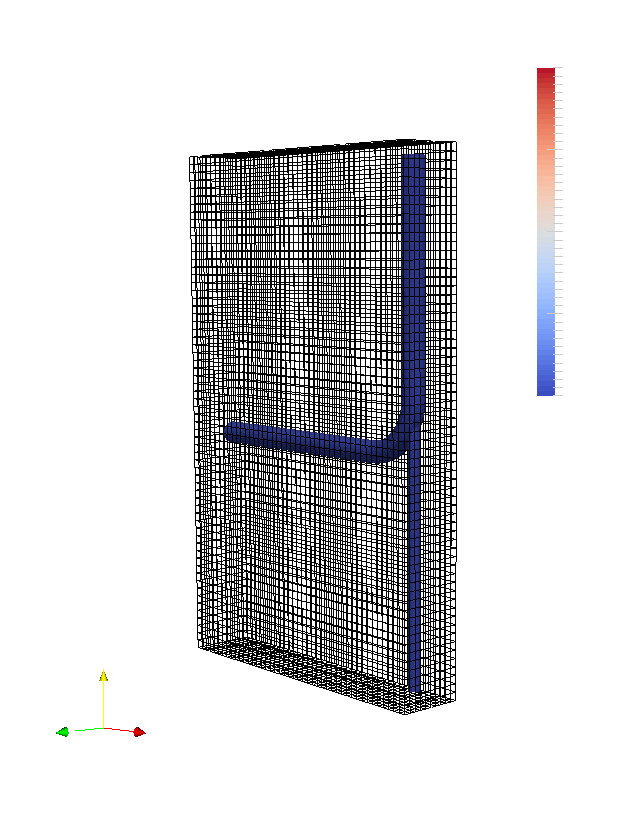
\includegraphics[scale=0.2]{mesh2.png}
\caption{Second mesh. Glando}
\end{figure}
\paragraph{}The values \lstinline!(44 64 10)! define the number of cells in the x, y and z respectively. When we've achieved a regular and dense enough mesh we must edit the lines below to have all the faces in the same type patch.
\begin{center}
\begin{lstlisting}
boundary
(
    frontAndBack
    {
        type patch;
        faces
        (
            (3 7 6 2)
            (1 5 4 0)
            (0 4 7 3)
            (2 6 5 1)
            (0 3 2 1)
            (4 5 6 7)
        );
    }
);
\end{lstlisting}
\end{center}
\paragraph{}The next step is to take \texttt{SnappyHexMesh} dictionary. Rather than create it, is better to take it from \texttt{openfoam4/applications/uilities/mesh/generation/\\snappyhexmesh} and paste it to the \texttt{Ypipe/system} folder. Inside the file there are a lot of comments and explanations about the mesh configuration and parameters (it's some kind of template).

\paragraph{}Let's see the geometry section of \texttt{snappyHexMeshDict}. It's possible to define an upper level of discretization inside our blockMesh using \texttt{searchableBox}. For this case is not necessary so we can delete it from the dictionary. Below, we must define all the solids we have in the problem. Every \texttt{.stl} file we have stored in the triSurface has to be specified here as follows. We can also include sub-solids in the same file, but we saved them in different files so the regions section should we empty.
\begin{center}
\begin{lstlisting}
geometry
{
    Inlet.stl
    {
        type triSurfaceMesh;
        regions
        {
        }
    }

    Inlet2.stl
    {
        type triSurfaceMesh;
        regions
        {
        }
    }

    Outlet.stl
    {
        type triSurfaceMesh;
        regions
        {
        }
    }

    Walls.stl
    {
        type triSurfaceMesh;
        regions
        {
        }
    }
    sphere2
    {
        type searchableSphere;
        centre  (1.5 1.5 1.5);
        radius  1.03;
    }
};
\end{lstlisting}
\end{center}

\paragraph{}\textbf{SnappyHexMesh} is one of the only meshers that can perform a parallel mesh of the domain (using multiple cores). This feature is enabled by \emph{castellatedMesh} feature. The parameter \texttt{maxLocalCells} and \texttt{maxGlobalCells} define the maximum number of cells per core and the maximum number of cells on the global mesh respectively. Another important parameter is the \emph{Surface based refinement}. Using this we can modify the maximum and minimum level of refinement of the solids. It detects when two surfaces are intersecting and let us apply an upper level of refinement to this edges. We have to define here all the solids as we've done before\footnote{It's important to include the full file name e.g. file.stl if we are dealing with separated files. If we work with regions only the patch name}.

\paragraph{}Lastly, we are going to modify the \texttt{locationInMesh} parameter. This define if we want to study the outside or the inside of the solid (and so we mesh the specified region of the domain). For this case we are going to study the flow inside the pipe so we put a point inside it (\texttt{(2.522222332 1.2324 0.0343)} is a good point) Now we save and close the file, and then type texttt{SnappyHexMesh} in the terminal window. The we can view the results by opening paraFoam.
